% \section{Định nghĩa, mô hình hoá bài toán}

% Bài toán mà chúng tôi thực hiện có tên là: Bài toán dự đoán tương tác xấu giữa hai thuốc với nhau. Cụ thể với bài toán này, đầu vào sẽ là một cặp thuốc, khi đó vấn đề chúng ta cần giải quyết là hai thuốc này có phản ứng xấu với nhau hay không. Ví dụ, thuốc Acetaminophen (Paracetamol) - một loại thuốc hạ sốt và giảm đau khi được sử dụng với Aldesleukin - một loại thuốc điều trị ung thư thì có thể làm tăng hoạt động gây độc cho gan của Acetaminophen. 

% Trong bài báo cáo này, chúng tôi sẽ mô hình hóa bài toán về dạng bài toán dự đoán liên kết giữa hai đỉnh trong đồ thị. Ở đây, mỗi đỉnh sẽ được nhúng vào một không gian vector 300 chiều, sau đó sử dụng mạng Conv-LSTM để dự đoán xem giữa hai đỉnh đấy có liên kết với nhau không.

% \section{Các vấn đề khó khăn, thách thức của bài toán}


% Các vấn đề khó khăn và thách thức của bài toán dự đoán tương tác thuốc-thuốc bao gồm:
% \begin{itemize}
%     \item \textbf{Dữ liệu không đồng nhất}: Dữ liệu về tương tác thuốc-thuốc thường không đồng nhất về cả định dạng khi thu thập dữ liệu từ nhiều nguồn khác nhau.

%     \item \textbf{Hạn chế về số lượng dữ liệu:} Dữ liệu về các tương tác thuốc-thuốc thường có hạn chế về số lượng và độ phong phú, làm giảm khả năng huấn luyện mô hình dự đoán chính xác.

%     \item \textbf{Phức tạp của mối quan hệ:} Mối quan hệ giữa các thuốc có thể phức tạp và đa dạng, với nhiều yếu tố ảnh hưởng như cơ chế tương tác, liều lượng, thời gian sử dụng, và đặc điểm bệnh lý của bệnh nhân.

%     \item \textbf{Tính hiếm gặp của tương tác:} Một số tương tác thuốc-thuốc có thể rất hiếm gặp hoặc ít được biết đến, điều này làm cho việc dự đoán trở nên khó khăn.

%     \item \textbf{Tính phi tuyến tính:} Một số tương tác thuốc-thuốc không tuân theo một mô hình tuyến tính, gây khó khăn trong việc dự đoán và hiểu quy luật của chúng.

%     \item \textbf{Dynamics:} Các tương tác thuốc-thuốc có thể thay đổi theo thời gian dựa trên sự thay đổi trong tình trạng sức khỏe của bệnh nhân hoặc sự điều chỉnh trong liều lượng.

%     \item \textbf{Đánh giá rủi ro:} Việc đánh giá rủi ro của các tương tác thuốc-thuốc đối với sức khỏe của bệnh nhân là một thách thức, đặc biệt là đối với các tương tác hiếm gặp hoặc không mong muốn.

% \end{itemize}

% Bên cạnh những khó khăn khách quan đó thì còn có khó khăn chủ quan là hạn chế về thiết bị huấn luyện mô hình để giải quyết bài toán. Cho nên trong bài báo cáo này, chúng tôi chỉ sử dụng dataset của drugbank để huấn luyện model.

% Ngoài ra, độ chính xác của model dự đoán tương tác thuốc cũng dựa vào khả năng nhúng của phương pháp nhúng đồ thị. Bởi vậy, ở trong báo cáo này chúng tôi sẽ sử dụng hai phương pháp nhúng là TransE và DistMult để cho thấy sự ảnh hưởng của phép nhúng đồ thị đến model dự đoán.

\section{Các phương pháp đánh giá kết quả}
% Bài toán về bản chất là bài toán phân loại nên nhóm nghiên cứu sẽ dựa trên 4 độ đo về hiệu quả mô hình phổ biến ở trong các bài toán phân loại đó là Accuracy, Precision, Recall và F1 Score. Cách tính và ý nghĩa của từng thang đo sẽ được đề cập tại phần sau

\subsection{Ma trận mâu thuẫn}
Ma trận mẫu thuẫn (Confusion Matrix) Là một phương pháp đánh giá kết quả của những bài toán phân loại với việc xem xét cả những chỉ số về độ chính xác và độ bao quát của các dự đoán cho từng lớp. Một confusion matrix gồm 4 chỉ số sau đối với mỗi lớp phân loại:

\begin{itemize}
    \item TP (True Positive): Số lượng dự đoán chính xác.
    \item TN (True Negative): Số lương dự đoán chính xác một cách gián tiếp. Ví dụ là khi mô hình dự đoán đúng một người phụ nữ không mang thai, tức là việc không chọn trường hợp người đó đang mang thai là đúnglà chính xác.
    \item FP (False Positive - Type 1 Error): Số lượng các dự đoán sai lệch. Ví dụ như khi mô hình dự đoán một người đàn ông đang mang thai và điều này là không thể xảy ra.
    \item FN (False Negative - Type 2 Error): Số lượng các dự đoán sai lệch một cách gián tiếp. Ví dụ ở đây là khi mô hình dự đoán một người phụ nữ đang mang bầu là không mang thai nhưng người đó chắc chắn là mang thai , tức là việc không chọn trường hợp không mang thai là sai. 
\end{itemize}

\begin{figure}[H]
    \centering
    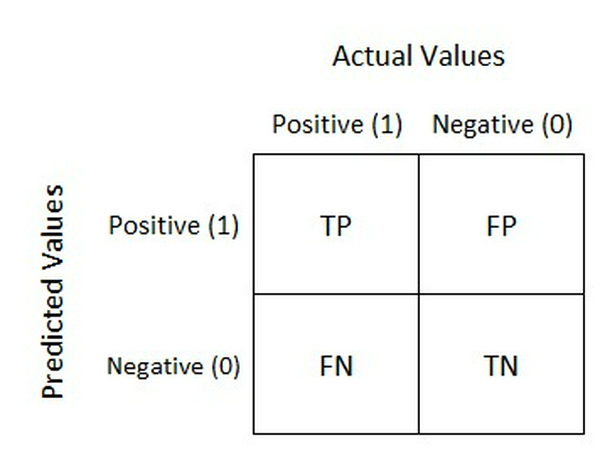
\includegraphics[scale = 0.5]{Images/confusion_matrix.jpg}
    \caption{Ma trận mâu thuẫn}
    \label{cofusion_matrix}
\end{figure}

\subsection{Accuracy} \label{accu}

Độ chính xác Accuracy đùng để tính toán tỉ lệ dự đoán đúng trên tổng số mẫu dự đoán là bao nhiêu. Chỉ số này càng cao tức là mô hình dự đoán càng đúng và càng tốt.

\[Accuracy = \frac{TP + TN}{TP + FP + FN + TN}\]

Accuracy là độ đo rất đơn giản và dễ hiểu dành cho các bài toán phân loại. Nhưng nhược điểm lớn nhất của độ đo này là khi mà dữ liệu mất cân bằng, có thể số dữ liệu của loại 1 vượt quá xa so với loại 2. Lúc này thì chỉ số chính xác này giường như là hiển nhiên. Để giải quyết các vấn đề này, các độ đo khác đã được dùng để đánh giá mô hình trong trường hợp dữ liệu mất cân bằng.

\subsection{Precision}
Precision cũng là một thang đo độ chính xác. Cụ thể trong tất cả các dự đoán Positive được đưa ra, bao nhiêu dự đoán là chính xác? Chỉ số này được tính theo công thức:

\[Precision = \frac{TP}{TP + FP}\]

Precision đo lường mức độ chính xác của kết quả đo lường và mức độ giữa các giá trị đo lường có thể lặp lại. Nếu một hệ thống có độ chính xác cao, nó có khả năng cung cấp các kết quả gần giống nhau khi được đo lường nhiều lần dưới điều kiện tương tự.

Trong một ngữ cảnh khác, trong lập trình và machine learning, thuật ngữ "precision" (độ chính xác) thường được sử dụng để mô tả tỷ lệ giữa số lượng các trường hợp dự đoán đúng của một lớp cụ thể và tổng số trường hợp dự đoán là positive cho lớp đó.

\subsection{Recall}

Độ đo Recall (còn được gọi là sensitivity hoặc true positive rate) là một độ đo đánh giá khả năng của một mô hình hoặc hệ thống trong việc bắt capture tất cả các trường hợp thực sự thuộc một lớp cụ thể. Độ đo này quan tâm đến khả năng của mô hình trong việc không bỏ sót các trường hợp dương thực sự (true positive). Công thức tính sẽ là: 

\[Recall = \frac{TP}{TP + FN}\]

\subsection{F-Score}
Để đánh giá độ tin cậy chung của mô hình, người ta đã kết hợp 2 chỉ số Precision và Recall thành một chỉ số duy nhất: F1-score, được tính theo công thức:

\[F\_score = \frac{2 * Recall * Precision}{Recall + Precision}\]

Một mô hình có chỉ số F-score cao chỉ khi cả 2 chỉ số Precision và Recall để cao. Một trong 2 chỉ số này thấp đều sẽ kéo điểm F-score xuống. Trường hợp xấu nhất khi 1 trong hai chỉ số Precison và Recall bằng 0 sẽ kéo điểm F-score về 0. Trường hợp tốt nhất khi cả điểm chỉ số đều đạt giá trị bằng 1, khi đó điểm F-score sẽ là 1.

Qua việc sử dụng chỉ số F-score, ta đã có một thước đo đáng tin cậy về hiệu năng của mô hình trong các bài toán phân loại, đặc biệt khi dữ liệu về một lớp lớn hơn gấp nhiều lần so với dữ liệu về lớp còn lại.

%     \item Các phương pháp giải quyết vấn đề lõi của bài toán
% \end{itemize}

\subsection{Area Under the Precision-Recall Curve (AUPR)}
Precision-Recall curve là một công cụ quan trọng trong việc đánh giá hiệu suất của mô hình phân loại, đặc biệt là trong các bài toán không cân bằng dữ liệu (imbalanced data). Nó biểu diễn mối quan hệ giữa precision (độ chính xác) và recall (độ phủ sóng) khi ngưỡng quyết định thay đổi.

Precision-Recall curve thường được sử dụng trong các tình huống mà các lớp cần được đánh giá không cân bằng, tức là một lớp có số lượng quan sát ít hơn so với lớp còn lại. Đường cong này cung cấp một cách để đánh giá hiệu suất của mô hình trên một loạt các ngưỡng quyết định khác nhau. Một điểm trên đường cong Precision-Recall tốt là điểm gần với góc trên bên trái của đồ thị, thể hiện một tỷ lệ cao của cả precision và recall.

\begin{figure}[H]
    \centering
    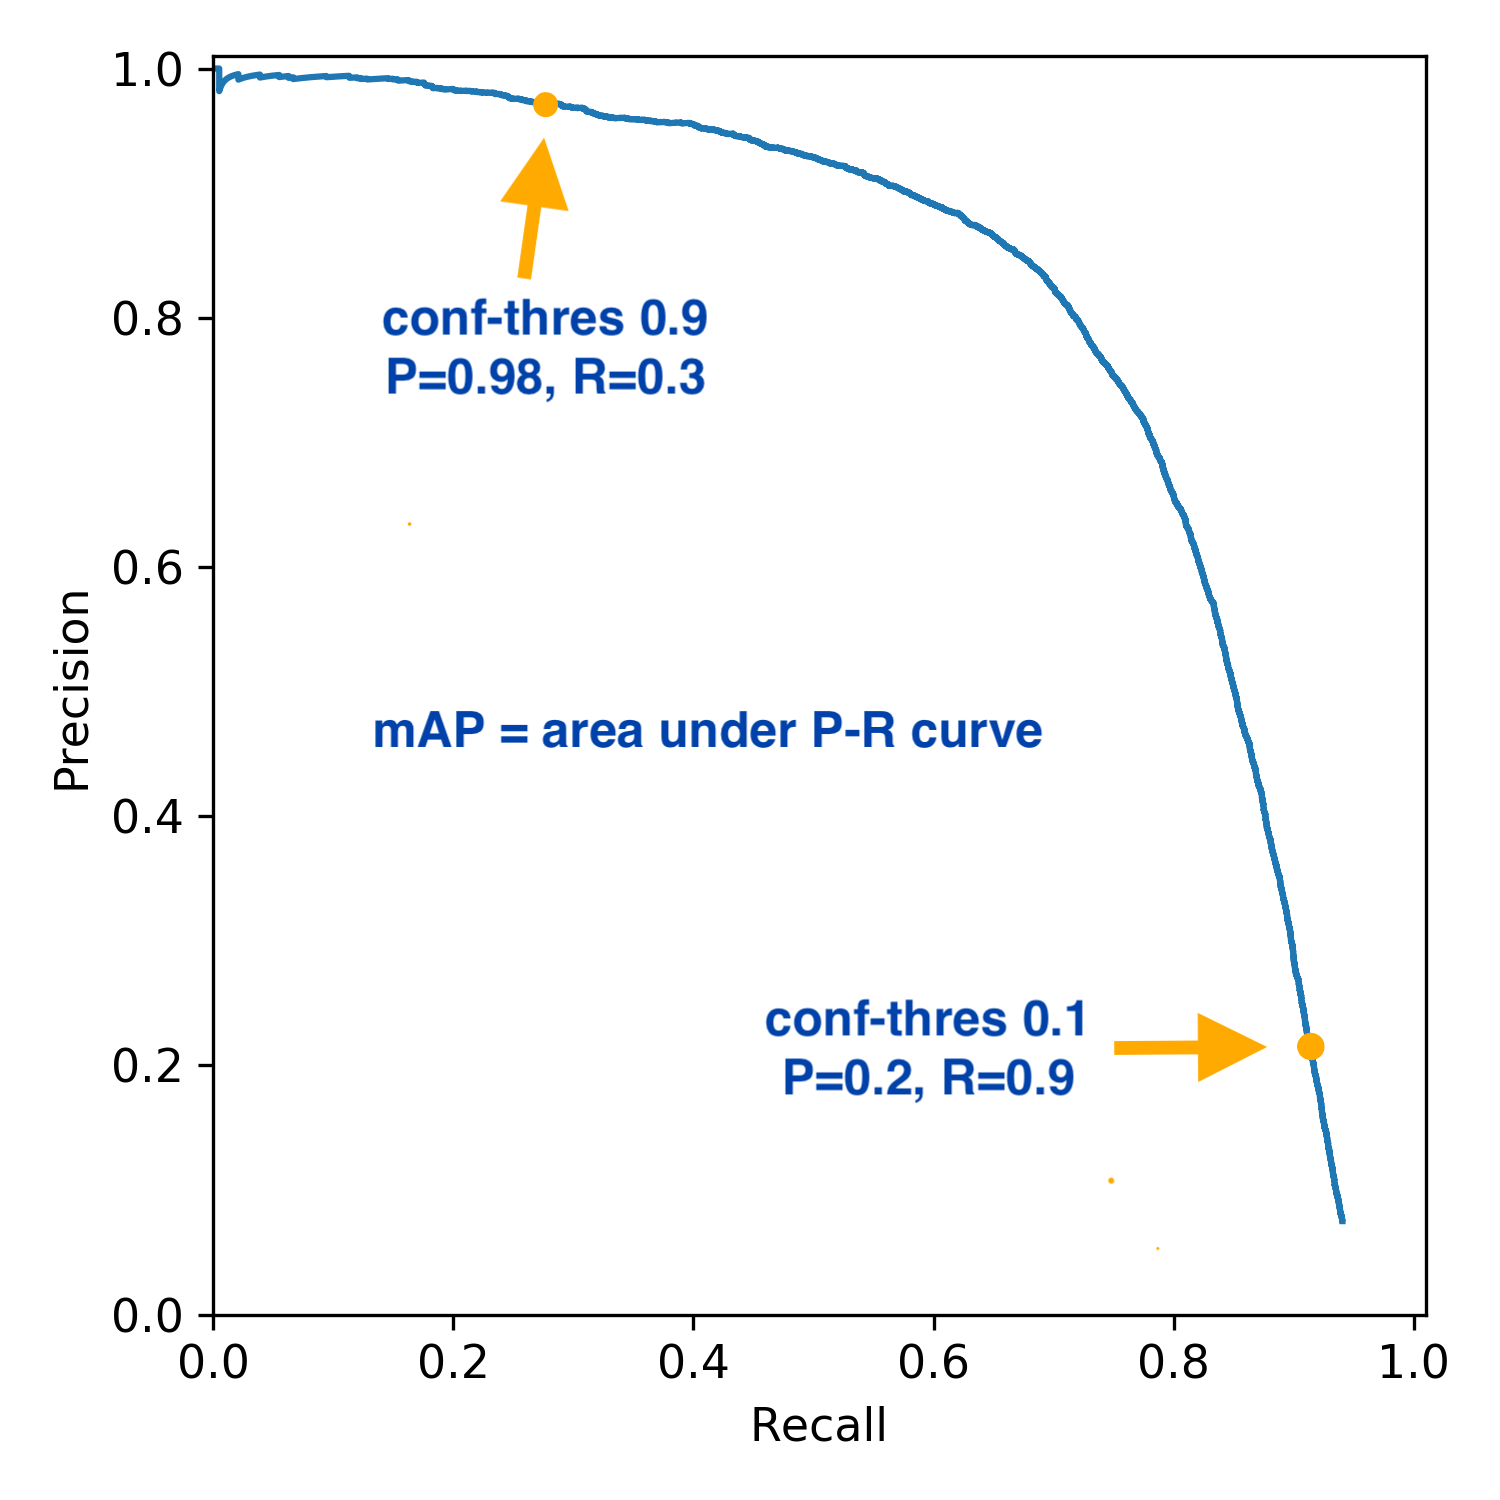
\includegraphics[width=0.7\linewidth]{Images/pr.png}
    \caption{Precision-Recall curve\cite{yolov3issue}}
    \label{pr_curve}
\end{figure}

Area Under the Precision-Recall curve (Diện tích dưới đường cong Precision-Recall), là một thước đo được sử dụng để đánh giá hiệu suất của một mô hình phân loại dựa trên độ chính xác và độ phủ sóng.

AUPR được tính từ diện tích dưới đường cong Precision-Recall để đo lường hiệu suất của mô hình.Giá trị AUPR càng cao, mô hình càng tốt. Nó thường được sử dụng trong các tình huống mà các lớp cần được đánh giá không cân bằng, nơi Precision-Recall curve là một công cụ đánh giá hiệu quả hơn so với ROC curve. Đặc biệt, khi có một số lượng lớn các mẫu âm tính và một số lượng nhỏ các mẫu dương tính, AUPR thường là lựa chọn hiệu quả.

\subsection{Matthews Correlation Coefficient}
Matthews Correlation Coefficient (Hệ số tương quan của Matthews), là một độ đo thường được sử dụng để đánh giá hiệu suất của một mô hình phân loại, đặc biệt trong các tình huống mà các lớp cần được đánh giá không cân bằng.

MCC tính toán một hệ số tương quan giữa dự đoán của mô hình và nhãn thực tế của dữ liệu, bằng cách sử dụng các giá trị True Positive (TP), True Negative (TN), False Positive (FP), và False Negative (FN). MCC có giá trị từ -1 đến +1, với +1 biểu thị một mô hình phân loại hoàn hảo, 0 biểu thị hiệu suất của một mô hình tương đương với dự đoán ngẫu nhiên, và -1 biểu thị một mô hình dự đoán hoàn toàn ngược lại so với thực tế.

Dưới đây là công thức của MCC:
$$\text{MCC} = \frac{TP \times TN - FP \times FN}{\sqrt{(TP + FP)(TP + FN)(TN + FP)(TN + FN)}}$$

% \section{Các công trình liên quan}

% Dự đoán tương tác thuốc-thuốc (DDI) là một vấn đề nghiên cứu quan trọng trong dược lý học, và đã có nhiều phương pháp được đề xuất để giải quyết vấn đề này bằng cách sử dụng các nguồn dữ liệu đa dạng. Truyền thống, công việc này dựa vào thí nghiệm in vitro và in vivo và tập trung vào các bộ cặp thuốc cụ thể với các hạn chế về phòng thí nghiệm.\cite{duke2012literature} Với sự xuất hiện của dữ liệu sinh học, các nhà nghiên cứu đã di chuyển sự chú ý đến việc tự động điền thông tin và hoàn chỉnh các knowledge graph sinh học bằng cách sử dụng các cơ sở dữ liệu có cấu trúc quy mô lớn và văn bản được công bố công khai. Các phương pháp này đã tạo ra nhiều knowledge graph sinh học, nhưng thường chứa dữ liệu không đầy đủ và không chính xác, gây trở ngại cho việc áp dụng chúng trong lĩnh vực phát triển thuốc an toàn.

% Gần đây, các phương pháp sử dụng máy học và khai thác văn bản đã được áp dụng, trong đó các đặc tính tương tự về dược lý của thuốc được sử dụng bằng cách coi nhiệm vụ dự đoán DDI là một vấn đề dự đoán liên kết. Các phương pháp khác nhau về đo lường độ tương tự của thuốc được sử dụng để suy luận DDI và các gợi ý liên quan của chúng. Tuy nhiên, các phương pháp dựa trên đặc tính chỉ dự đoán các DDI nhị phân hoặc những DDI đã được xác định trước trong các cơ sở dữ liệu có cấu trúc và gặp khó khăn do tính thưa dữ liệu và yêu cầu tính toán lớn.

% Các phương pháp mới trong dự đoán tương tác thuốc-thuốc (DDI) sử dụng hai kỹ thuật chính là knowledge graph (KGs) và embedding văn bản để giải quyết các thách thức về dữ liệu không đầy đủ và thưa thớt. Trong đó, embedding đồ thị là một công cụ mạnh mẽ được sử dụng để biểu diễn các thực thể và mối quan hệ trong KGs dưới dạng vector, ví dụ như TransE, TransD, TransH, HolE.\cite{main-paper} Các phương pháp này sử dụng embedding để mô hình hóa mối tương tác giữa các thuốc dựa trên thông tin về mối quan hệ và đặc điểm của chúng trong KGs.

% Ngoài ra, một số phương pháp cũng sử dụng khai thác văn bản để dự đoán và đánh giá DDI mới bằng cách trích xuất thông tin về thuốc từ văn bản khoa học hoặc tự động suy luận DDI từ các tài liệu MEDLINE.\cite{kastrin2018predicting, percha2013informatics, tatonetti2012data}

% Sự kết hợp của đa nguồn dữ liệu và kiến thức về thuốc trong một Knowledge Graph là một phần quan trọng của các phương pháp này. Điều này giúp tạo ra các biểu diễn chất lượng cao về các mối quan hệ và đặc điểm của thuốc, từ đó cung cấp thông tin hữu ích cho việc dự đoán DDI.

% Mặc dù cách thức trích xuất DDI và các dự đoán được thực hiện khác nhau giữa các phương pháp. Nhiều cách tiếp cận đã trích xuất DDI từ văn bản y sinh bằng cách sử dụng kiến thức phong phú và các đặc điểm nghèo kiến thức\cite{hailu2013ucolorado} hoặc từ từ vựng, cú pháp và các đặc trưng dựa trên ngữ nghĩa.\cite{bobic2013scai} Các cách tiếp cận khác, tập trung vào việc phân loại DDI trong đó SVM được huấn luyện bằng cách sử dụng các tính năng của thuốc được tạo bằng các biện pháp tương tự\cite{bjorne2013uturku, rastegar2013uwmtiads} hoặc bằng cách khai thác thông tin ngôn ngữ.\cite{chowdhury2013fbkirst} Ngoài ra, các cách tiếp cận khác đã sử dụng văn bản khai thác để trích xuất DDI từ kho văn bản có chú thích ngữ nghĩa các tài liệu mô tả DDI từ các bản tóm tắt của DrugBank và MEDLINE.\cite{herrero2013ddi, segura2014lessons}

\newpage